\documentclass[12pt]{article}
\usepackage{tikz-qtree}
\usepackage[cm]{fullpage}
\usepackage{tipa}

\begin{document}
\title{\Huge Agreement in German}
\author{Charles Redmon (M.A. '14, H-1499)}
\date{}
\maketitle
\begin{flushleft}
The following work is an exercise in examining the ways in which agreement patterns in German must be accounted for in a Minimalist conception of syntactic structure. In visualizing the tree structures, I have chosen to show only those most relevant features for the topic at hand. Where I find such choices may lead to some confusion, I have done my best to clarify the issues in the adjoining discussion. Many aspects of German syntax are still unclear to me, so much of the analysis presented below will be mixed with necessary caveats and questions for further speculation. It may very well be understood that any investigation of Minimalist syntax requires reference to Chomsky's (1995) {\it Minimalist Program}, nevertheless it is worth noting here that all foregoing theoretical considerations are drawn loosely from this text \cite{chomsky}. And finally, in selecting sample sentences to model I have chosen to draw on Jacob \& Wilhelm Grimm's ``H\textipa{\"a}nsel und Gretel,'' originally published in the 1812 collection, {\it Kinder- und Hausm\textipa{\"a}rchen} \cite{grimm}.  It is hoped that such a choice will make for more interesting reading and a welcome departure from the ``John loves Mary'' (or "Johann liebt Marie") trope. 

\section{German Agreement: Core Relations}
Agreement in German can be divided into two major types: DP-internal and external, Subject-Verb agreement. As Subjects ultimately ought to be analyzed as Determiner Phrases, it seems appropriate to begin with the former. An awareness of DP-internal agreement will also become helpful later when Verb case checking in the Agr$_s$ Spec-Head relation accounts for complete agreement in DP-internal case inflections. 
\subsection{DP-internal Agreement}
The set of $\phi$-features active in German agreement comprises the typical Person-Number-Gender categories. There are of course various nuances to these categories, such as the fact that Subject-Verb agreement only Person and Number are active (and therefore represented morphologically), while case inflection requires reference to all three, but in general the system is organized as follows: Person \{1st, 2nd (+/- honorific), 3rd\}, Number \{singular, plural\}, Gender \{feminine, masculine, neuter\}. I will not go into all the morphological manifestations of these categories here, but will note them as they appear in examples below. German, like English, has requisite definite articles for common nouns (note: the orthography of German capitalizes all nouns, regardless of common or proper status), and when adjectives are included in the DP both the article and the adjective modifying the noun are inflected according to the $\phi$-features of that noun. This pattern may be conceptually simple in a broad sense, but we will see in the examples below that working out such agreement features in the larger architecture of Minimalism poses some distinct challenges. All other disclaimers aside, we can begin to see the kind of structure required in the first example. In Figure 1a, we have the phrase "die armen Kinder" ('the poor children'), where {\it Kinder} is the plural of {\it das Kind}, a neuter noun, and the article and adjective ({\it die} and {\it armen}, respectively) are inflected for plural Number and nominative Case (the plural in this case has its own inflection regardless of gender of the base noun).\\
\bigskip
{\bf Figure 1a. ``die armen Kinder"} \\
\bigskip
{\centering
\begin{tikzpicture}
\Tree [.Agr$_N$P 
		Spec [.Agr$_N$$'$ 
		Agr$_N$ [.Agr$_N$P 
		Spec [.Agr$_N$$'$ 
		Agr$_N$ [.DP
		[.D {$die$} ] [.AdjP 
		[.A {$armen$} ] [.NP
		[.N {$Kinder$} ] ] ] ] ] ] ] ]
\end{tikzpicture}\\
}

{\bf Figure 1b. ``die armen Kinder'' (Adjective-Noun Agr)} \\
\bigskip
{\centering
\begin{tikzpicture}
\Tree [.Agr$_N$P 
		Spec [.Agr$_N$$'$ 
		Agr$_N$ [.Agr$_N$P 
		[.Spec \node(NP){$Kinder_i$}; ] [.Agr$_N$$'$ 
		[.Agr$_N$ \node(a){$armen_j$}; Agr$_N$ ] [.DP
		[.D {$die$} ] [.AdjP 
		[.A \node(tj){$t_j$}; ] [.NP
		[.N \node(ti){$t_i$}; ] ] ] ] ] ] ] ]
\draw[semithick, ->] (ti)..controls +(south west:4) and +(south:3)..(NP);
\draw[dashed, ->] (tj)..controls +(south west:2) and +(south:2)..(a);
\end{tikzpicture}\\
}
\bigskip
In the base structure (Figure 1a) I have located the Determiner Phrase within a complex of two Agr$_N$Ps, adopting the mnemonic convention from Agr$_s$/Agr$_o$, where the subscript refers to the category of the item moving into Spec (and therefore the item to which the category adjoining to Agr conforms). It could be argued that Agr$_{NP}$ might in fact be a more proper characterization, but as this is just a mnemonic and NP=N in this example, I leave this as a trivial notational matter. In Figure 1b, we see the movements responsible for Adjective-Noun agreement, with the noun {\it Kinder} moving into Spec of the lower Agr$_N$P and the adjective {\it armen} adjoining to Agr$_N$ to check its $\phi$-features. We then get the same movement pattern in Figure 1c for Determiner-Noun agreement, with {\it Kinder} moving again in cyclic fashion to Spec of the higher Agr$_N$P and the article {\it die} moving up to adjoin with Agr$_N$ and undergo the same feature-checking process. \\
\bigskip
{\bf Figure 1c. ``die armen Kinder'' (Determiner-Noun Agr)} \\
\bigskip
{\centering
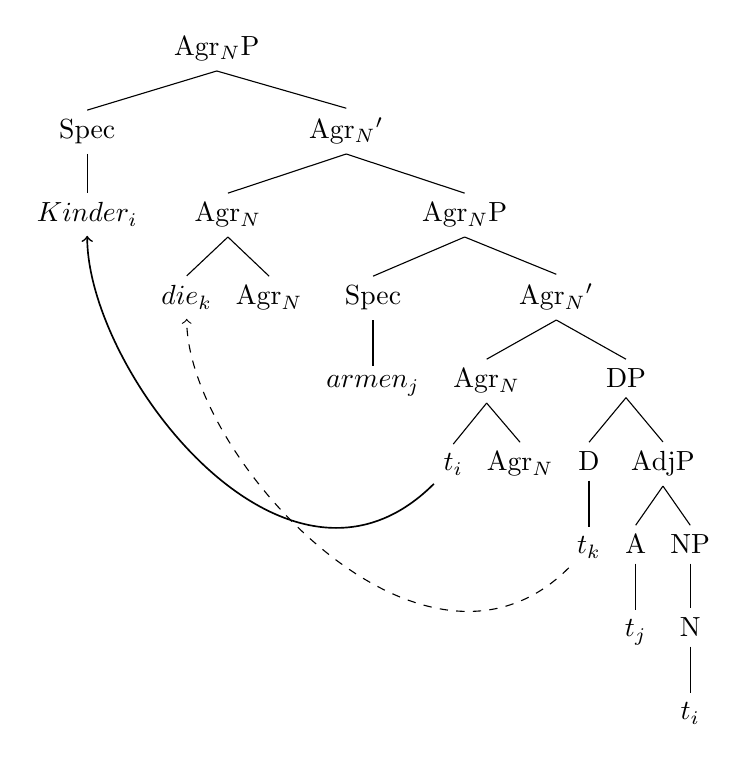
\begin{tikzpicture}
\Tree [.Agr$_N$P 
		[.Spec \node(NP){$Kinder_i$}; ]
		[.Agr$_N$$'$ [.Agr$_N$ \node(d){$die_k$}; Agr$_N$ ]
		[.Agr$_N$P [.Spec {$armen_j$} ]
		[.Agr$_N$$'$ [.Agr$_N$ \node(ti){$t_i$}; Agr$_N$ ] [.DP
		[.D \node(tk){$t_k$}; ] [.AdjP 
		[.A {$t_j$} ] [.NP
		[.N {$t_i$} ] ] ] ] ] ] ] ] ] 
\draw[semithick, ->] (ti)..controls +(south west:3) and +(south:2)..(NP);
\draw[dashed, ->] (tk)..controls +(south west:3) and +(south:2)..(d);
\end{tikzpicture} \\
}
\bigskip
In the local case, where we only focus on the constituents of the DP, the above characterization of agreement poses no great problems. Conceptually, the cyclic movement of the Noun through both Agreement Phrases, at each step undergoing a feature-checking process with the remaining constituents of the DP,  mirrors that which has more broadly been conceived for the clause; however, when we consider the place and requisite movements of DPs at a wider scale the current arrangement poses notable problems. For one, because of the nature of Agreement relations in Minimalist syntax, which place the Noun in the Spec position above the adjective and article/determiner, we are forced to consider DP-internal agreement to be 'covert' process (i.e. after Spellout), so that the order `pronounced' is the initial order as shown in Figure 1a: Det-Adj-Noun. Yet this appeal to LF still does not resolve the question of how to treat the DP as a unit in larger syntactic processes. For reasons to be addressed later, when the verb is forced to move for Tense (i.e. when Tense is not occupied by an Auxiliary of some sort) Subject-Verb agreement checking (and by extension Object-Verb checking) must happen in the overt syntax, and since the constituent structure of Subject and Object is ultimately that of a DP, the DP must be able to carry its agreement structure with it as a unit. This requirement suggests that Agr$_N$P must in fact be internal to the DP, a structure which is loosely conceived in Figure 1d; however, as yet I am not clear on the present arrangement. The requirement for upward movement necessitates either a double-DP structure of the kind shown or a splitting of the intermediate node (D$'$) into two, one above and one below the Agr$_N$P complex. As I am less clear on the consequences of a D$'$ split, I have chosen to adopt the former solution. \\
\bigskip 
{\bf Figure 1d. ``die armen Kinder'' (DP-internal Agr)} \\
\bigskip
{\centering
\begin{tikzpicture}
\Tree [.DP 
		D [.{\ldots} 
		[.Agr$_N$P Spec
		[.Agr$_N$$'$ Agr$_N$
		[.Agr$_N$P Spec
		[.Agr$_N$$'$ Agr$_N$ [.DP
		[.D {$die$} ] [.AdjP 
		[.Adj {$armen$} ] [.NP
		[.N {$Kinder$} ] ] ] ] ] ] ] ] ] ]
\end{tikzpicture}\\
}
\bigskip
In summary, DP-internal agreement happens later (in LF, to use the GB conception), but the structure required for such agreement feature checking must be contained within the DP so that we do not require the derivation-specific construction of Agreement Phrases at each terminal location of DPs in the main clause. And so while the technical matters of incorporating agreement structure into the DP are unclear to me at the moment, there is clear motivation for this inclusion; it suggests the structure within the DP is relatively unchanging and no appeal to external structures is required to explain the agreement between constituents of the Determiner Phrase.\\
\subsection{Predicate Adjectives}
An interesting consequence of the DP-internal agreement structure is its prediction that adjectives outside of the Determiner Phrase will lack agreement with the NP, a prediction which is indeed borne out in German. Thus while DP-internal adjectives are inflected for agreement with the NP complement, predicate adjectives are given in an un-inflected `base' form. And so regardless of the Gender or Number of the noun which they serve to modify, the form of a predicate adjective will remain the same. For example, taking our initial phrase ``die armen Kinder" and converting it into a predicate adjective structure of the form ``The children are poor'' yields the sentence: ``Die Kinder sind arm.'' (Figure 1e).\\
\newpage
{\bf Figure 1e. ``Die Kinder sind arm." (base)}\\
{\centering
\bigskip
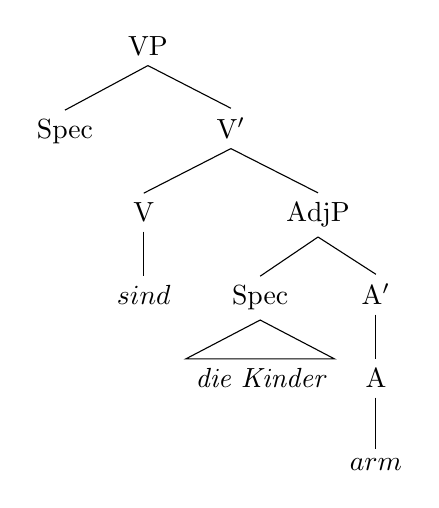
\begin{tikzpicture}
\Tree [.VP
		Spec  [.V$'$
		[.V {$sind$} ] [.AdjP
		[.Spec \edge[roof];{\it die Kinder} ] [.A$'$
		[.A {$arm$} ] ] ] ] ]	
\end{tikzpicture}\\
}
\bigskip
From the above structure we of course expect {\it die Kinder} to move upward to occupy Subject position and check agreement with the verb {\it sind}, which is inflected for 3rd person plural. These movements will yield the ultimate word order we require (i.e. "Die Kinder sind arm."). And while there are some notable differences in the Noun-Adjective arrangement in this structure as compared with the earlier case -- namely that the DP {\it die Kinder} occupies the Spec position rather than the complement position of the Adjective, a configuration which is motivated largely by the DP's need for theta-role assignment from the adjective -- the critical departure is that the adjective and noun are no longer in the same DP, and given our earlier claim that Noun-Adjective agreement is DP-internal, this configuration accounts for the lack of agreement we find in predicate adjectives. 
\subsection{Subject-Verb Agreement}
The process in German whereby a verb checks its $\phi$-features for agreement with the subject (and correspondingly checks for nominative case on the subject) conforms with the convention set out in Chomsky (1995). That is, the Subject moves to Spec of Agr$_s$P while the Verb adjoins with the head (Agr$_s$), and from this configuration the aforementioned checking processes commence. For example, in Figure 2a(i) we have the base structure of ``Gretel weinte bittere Tr\textipa{\"a}nen.'' ('Gretel cried bitter tears.'). \\
\bigskip
{\bf Figure 2a(i). ``Gretel weinte bittere Tr\textipa{\"a}nen.'' (base)} \\
\bigskip
{\centering
\begin{tikzpicture}
\Tree [.VP [.Spec {$Gretel$} ] 
		[.V$'$ [.DP D [.AdjP [.A {$bittere$} ] [.NP [.N {$Tr\textipa{\"a}nen$} ] ] ] ] 
			[.V {$weinte$} ] ] ]
\end{tikzpicture} \\
}
As can be seen from the VP-internal structure, {\it weinte} ('cried') takes the object {\it bittere Tr\textipa{\"a}nen} ('bitter tears'), which will in fact be checked for accusative case in an Agr$_o$P not shown in Figure 2a(ii). I only note this here that in focusing on Subject-Verb agreement, which is a two-fold process (as opposed to just case checking in the case of the Object), I have left out some necessarily prior processes. But of course, since the verb cannot move back down the tree after adjoining to Agr$_s$ I assume the adjoining to Agr$_o$ (as well as later adjoining to Tense) has already occured (meaning that the movement arrow straight to Agr$_s$ from V would more accurately have multiple 'pit stops' along the way). In Figure 2b(i) we examine the present perfect form of this sentence: ``Gretel hat bittere Tr\textipa{\"a}nen geweint." ('Gretel has cried bitter tears.'), where the auxiliary verb {\it hat} is projected from the head of the TP. \\
\bigskip
{\bf Figure 2a(ii). ``Gretel weinte bittere Tr\textipa{\"a}nen.'' (S-V Agr)} \\
\bigskip
{\centering
\begin{tikzpicture}
\Tree [.Agr$_s$P 
		[.Spec \node(s){$Gretel_i$}; ] [.Agr$_s$$'$ 
		[.Agr$_s$ \node(v){$weinte_j$}; Agr$_s$ ] [.{\ldots} 
		[.VP [.Spec \node(ti){$t_i$}; ] 
		[.V$'$ [.DP D [.AdjP [.A {$bittere$} ] [.NP [.N {$Tr\textipa{\"a}nen$} ] ] ] ] 
		[.V \node(tj){$t_j$}; ] ] ] ] ] ]
\draw[semithick, ->] (ti)..controls +(south west:3) and +(south:2)..(s);
\draw[dashed, ->] (tj)..controls +(south west:3) and +(south:2)..(v);
\end{tikzpicture} \\
}

{\bf Figure 2b(i). ``Gretel hat bittere Tr\textipa{\"a}nen geweint." (base)} \\
\bigskip
{\centering
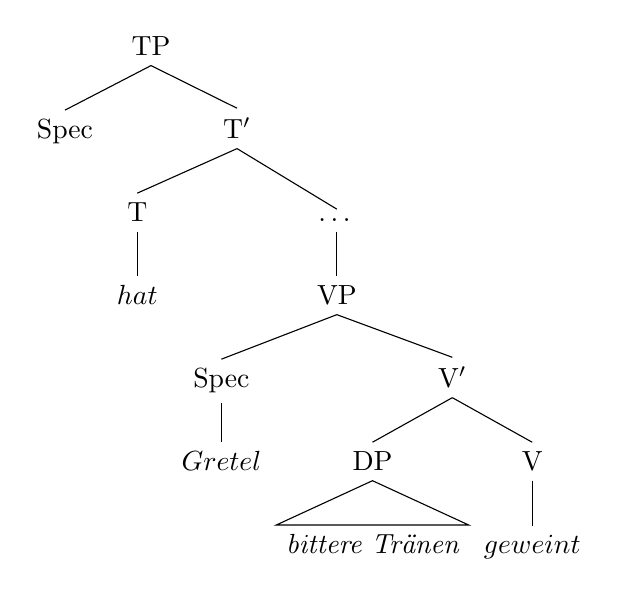
\begin{tikzpicture}
\Tree [.TP Spec [.T$'$ 
	[.T {$hat$} ] [.{\ldots}
	[.VP [.Spec {$Gretel$} ] 
	[.V$'$ [.DP \edge[roof]; {\it bittere Tr\textipa{\"a}nen} ] [.V {$geweint$} ] ] ] ] ] ] ] ]
\end{tikzpicture} \\
}
Because the V-feature of Tense is already satisfied by the auxiliary, there is no motivation for overt movement of the main verb {\it geweint} (although I assume this verb will also have to check tense later by some process of adjoining to T, which it does after checking the Object's case, also a covert process when not under pressure to satisfy Tense's V-feature). And so the auxiliary {\it hat} adjoins to Agr$_s$ and checks agreement with the Subject {\it Gretel}, which has moved into Spec of Agr$_s$P (Figure 2b(ii)).\\
\bigskip
{\bf Figure 2b(ii). ``Gretel hat bittere Traenen geweint.'' (Subject-Aux Agr)} \\
\bigskip
{\centering
\begin{tikzpicture}
\Tree [.Agr$_s$P 
		[.Spec \node(s){$Gretel_i$}; ] [.Agr$_s$$'$
		[.Agr$_s$ \node(aux){$hat_j$}; Agr$_s$ ] [.TP 
		Spec [.T$'$ 
		[.T \node(tj){$t_j$}; ] [.{\ldots}
		[.VP [.Spec \node(ti){$t_i$}; ] 
		[.V$'$ [.DP \edge[roof]; {\it bittere Tr\textipa{\"a}nen} ] 
		[.V {$geweint$} ] ] ] ] ] ] ] ]
\draw[semithick, ->] (ti)..controls +(south west:4) and +(south:3)..(s);
\draw[dashed, ->] (tj)..controls +(south west:2) and +(south:2)..(aux);
\end{tikzpicture} \\
}
\bigskip
These relations constitute the core features of agreement in German, but they are by no means sufficient for description of the system as a whole. In that regard I have left many things out, some of which will be covered in the next section. As a brief preview of the major issues which remain to be addressed, we still have not touched on motivations for the base constituent order (internal to the VP) in German, nor have we delved into the ubiquitous Verb-Second (V2) phenomenon. To exemplify these and other syntactic relations I now look to a selection of miscellaneous sentences from ``H\textipa{\"a}nsel und Gretel,'' each syntactically enlightening (and perhaps non-syntactically self-indulgent) in a different way. 
\section{Sentences from ``H\textipa{\"a}nsel und Gretel''}
The first sentence to be examined in this section was chosen initially as a demonstration of Wh-movement in German, but as it turns out no Wh-movement is possible without also pulling the verb into second position and thereby exemplifying V2 structure as well. And so in Figure 3a we have ``Wie sollen wir aus dem Wald kommen?'' ('How should we come out of the forest?'), where {\it wie} is the Wh-word 'how', and {\it sollen} is the modal verb 'should', whose main verb {\it kommen} ('to come') consequently remains at the very end of the clause. \\
{\bf Figure 3a. ``Wie sollen wir aus dem Wald kommen?''}\\
\bigskip
{\centering
\begin{tikzpicture}
\Tree [.TP
		Spec [.T$'$ 
		[.T {$sollen$} ] [.Agr$_o$P
		Spec [.Agr$_o$$'$ 
		Agr$_o$ [.AdvP
		[.Adv {$wie$} ] [.VP
		[.Spec {$wir$} ] [.V$'$
		V [.VP
		[.PP \edge[roof];{\it aus dem Wald} ] [.V$'$
		[.V {$kommen$} ] ] ] ] ] ] ] ] ] ]
\end{tikzpicture} \\
}
\bigskip
There is a complex series of movements to be made here, but I have chosen to focus on only those movements which are overt and therefore affect the output word order. I assume, as I noted before, that the main verb (as well as the Prepositional Phrase modifier) will ultimately move out of the VP for agreement feature checking, which in this complex VP means that {\it kommen} first moves to the higher V, but these are too many issues to be addressed in one tree. I turn then to the (overtly) active members of the base structure: {\it sollen}, {\it wie}, and {\it wir} ('we'; Subj). First, note that the modal verb is projected from the same position as the auxiliary from the previous example: i.e. the head of TP. This will have important consequences for {\it sollen}'s like behavior in S-V agreement and the corresponding relegation of {\it kommen} to clause-final position. Looking to the Subject, the position of {\it wir} is typical and uncontroversial; {\it wie}, on the other hand, has been analyzed as an adverb outside of the VP, but while it may be argued that the Wh-word ought to be closer to the verb, I don't see any principled arguments in favor one over the other. Since the end result is movement to Spec of CP, the effect of the locus of that movement is not clear to me. For visualization of these movements we turn to Figure 3b (note the ordering of subscripts and coloring of lines is not meant to indicate movement order or any other such relations). Movements to Agr$_s$P are just as we saw in the previous example, and the movement of {\it wie} to Spec of CP is again as expected from conventional Minimalist structure. The more interesting consequence of Wh-movement is that it requires projection of a CP, which I claim is the sole structure responsible for the V2 pattern in German. Turning to Figure 3c, after checking agreement in Agr$_s$P, the auxiliary then moves to the head of CP, just as in English. This Subject-Aux inversion in Wh-questions may seem unremarkable from the standpoint of English, but what we find in German is that all kinds of adverbial adjuncts and topicalizations trigger the same movement and the same inversion, the end result being that the verb always comes second in German word order.\\
\newpage
{\bf Figure 3b. ``Wie sollen wir aus dem Wald kommen?'' (S-Aux Agr; Wh-movement)} \\
\bigskip
{\centering
\begin{tikzpicture}
\Tree [.CP 
		[.Spec \node(wh){$wie_i$}; ] [.C$'$ 
		C [.Agr$_s$P 
		[.Spec \node(s){$wir_k$}; ] [.Agr$_s$$'$
		[.Agr$_s$ \node(aux){$sollen_j$}; Agr$_s$ ] [.TP
		Spec [.T$'$ 
		[.T \node(tj){$t_j$}; ] [.{\ldots}
		[.AdvP
		[.Adv \node(ti){$t_i$}; ] [.VP 
		[.Spec \node(tk){$t_k$}; ] [.V$'$ 
		V [.VP \edge[roof];{\it aus dem Wald kommen} ] ] ] ] ] ] ] ] ] ] ] ]
\draw[dashed, ->] (ti)..controls +(south west:4) and +(south:4)..(wh);
\draw[semithick, ->] (tk)..controls +(south west:4) and +(south:4)..(s);
\draw[semithick, ->] (tj)..controls +(south west:2) and +(south:2)..(aux);
\end{tikzpicture}\\
}
\bigskip
\newpage
{\bf Figure 3c. ``Wie sollen wir aus dem Wald kommen?'' (Final Aux-movement)} \\
\bigskip
{\centering
\begin{tikzpicture}
\Tree [.CP 
		[.Spec {$wie_i$} ] [.C$'$ 
		[.C \node(aux){$sollen_j$}; ] [.Agr$_s$P 
		[.Spec {$wir_k$} ] [.Agr$_s$$'$
		[.Agr$_s$ \node(tj){$t_j$}; Agr$_s$ ] [.TP
		Spec [.T$'$ 
		[.T {$t_j$} ] [.{\ldots}
		[.AdvP
		[.Adv {$t_i$} ] [.VP 
		[.Spec {$t_k$} ] [.V$'$ 
		V [.VP \edge[roof];{\it aus dem Wald kommen} ] ] ] ] ] ] ] ] ] ] ] ]
\draw[semithick, ->] (tj)..controls +(south west:2) and +(south:2)..(aux);
\end{tikzpicture}\\
}
\bigskip
In the next sentence, we see the behavior of one such V2-inducing topicalization: ``Als der Mond kam, machten sie sich auf." ('As the moon came, they got themselves up.'). Here the topic (a CP, with only relevant aspects of its structure shown) has moved into Spec of the larger CP, the assumption being that a more basic or earlier structure had the CP {\it als der Mond kam} ('as the moon came') as a lower embedded clause. The VP structure is largely the same as we have seen in other examples, only that here the object of V is a reflexive anaphor {\it sich} ('themselves'), and the Verb has a complex {\it auf + machten} form. The infinitival form of the verb is actually {\it aufmachen}, although I'm unsure whether {\ auf} ('on/up') is an affix or rather a kind of clitic. The clitic argument seems stronger because we also get constructions like {\it aufgemacht} ('got up'; Past Participle), where the {\it auf} retains peripheral location; however I am unsure of how such a structure would be organized so I have left it opaque here. The main result which has to follow from any analysis is that {\it machten} moves for Tense, leaving the {\it auf} at the end of the clause. Subject-Verb agreement movements then happen as shown earlier, in the usual Agr$_s$P configuration. Then because the topicalization of {\it als der Mond kam} projects a higher-up CP, the tensed verb {\it machten} must move higher up into C. This movement yields the requisite order and aligns with other such CP-driven configurations which are responsible for the V2 structure. As yet I don't have a compelling argument for {\it why} tensed, subject-agreeing verbs move into C; there is only the theoretical motivation for encompassing the V2 pattern in a single structure and series of movements. Since the pattern at a surface level is the same for Wh-questions, clause-initial adverbial phrases, and other more complex topicalizations, this is an appealing result. Still, what is 'appealing' may not be theoretically tenable in a larger sense, so I welcome such criticisms. \\
\newpage
{\bf Figure 4a. ``Als der Mond kam, machten sie sich auf.''}\\
\bigskip
{\centering
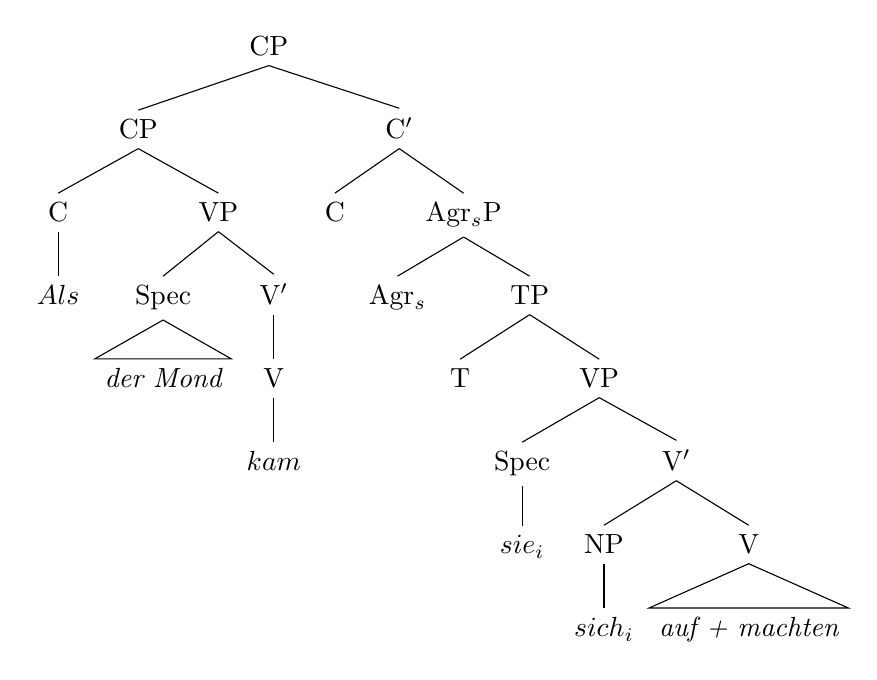
\begin{tikzpicture}
\Tree [.CP 
		[.CP [.C {$Als$} ] [.VP
		[.Spec \edge[roof];{\it der Mond} ] [.V$'$
		[.V {$kam$} ] ] ] ] [.C$'$ 
		C [.Agr$_s$P 
		Agr$_s$ [.TP
		T [.VP
		[.Spec {$sie_i$} ] [.V$'$
		[.NP {$sich_i$} ] [.V \edge[roof];{\it auf + machten} ] ] ] ] ] ] ]
\end{tikzpicture}\\
}
\bigskip
\bigskip
\bigskip
\bigskip
\bigskip
{\bf Figure 4b. ``Als der Mond kam, machten sie sich auf.'' (S-V Agr)}\\
\bigskip
{\centering
\begin{tikzpicture}
\Tree [.CP 
		[.CP [.C {$Als$} ] [.VP
		[.Spec \edge[roof];{\it der Mond} ]  [.V$'$
		[.V {$kam$} ] ] ] ] [.C$'$ 
		C [.Agr$_s$P 
		[.Spec \node(s){$sie_i$}; ] [.Agr$_s$$'$
		[.Agr$_s$ {$machten_j$} Agr$_s$ ] [.TP
		T [.VP
		[.Spec \node(ti){$t_i$}; ] [.V$'$
		[.NP {$sich$} ] [.V \edge[roof];{\it auf + $t_j$} ] ] ] ] ] ] ] ]
\draw[semithick, ->] (ti)..controls +(south west:4) and +(south:3)..(s);
\end{tikzpicture}\\
}
\newpage
{\bf Figure 4c. ``Als der Mond kam, machten sie sich auf.'' (Verb movement to CP-head)}\\
\bigskip
{\centering
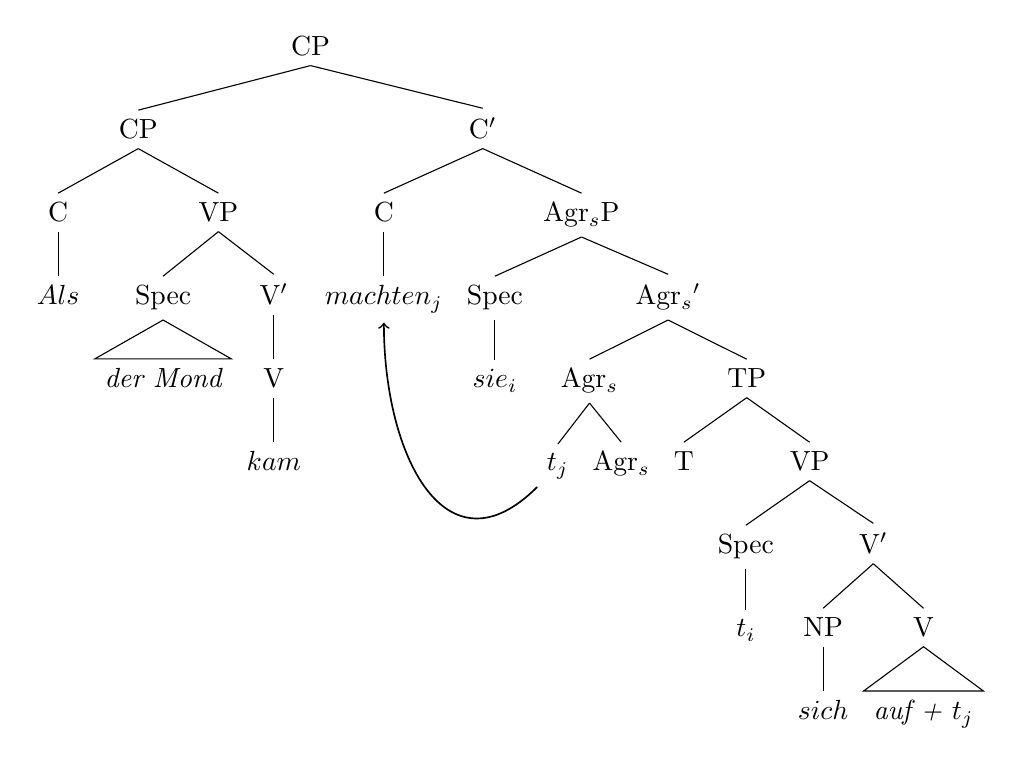
\begin{tikzpicture}
\Tree [.CP 
		[.CP [.C {$Als$} ] [.VP
		[.Spec \edge[roof];{\it der Mond} ]  [.V$'$
		[.V {$kam$} ] ] ] ] [.C$'$ 
		[.C \node(v){$machten_j$}; ] [.Agr$_s$P 
		[.Spec {$sie_i$} ] [.Agr$_s$$'$
		[.Agr$_s$ \node(tj){$t_j$}; Agr$_s$ ] [.TP
		T [.VP
		[.Spec {$t_i$} ] [.V$'$
		[.NP {$sich$} ] [.V \edge[roof];{\it auf + $t_j$} ] ] ] ] ] ] ] ]
\draw[semithick, ->] (tj)..controls +(south west:2) and +(south:2)..(v);
\end{tikzpicture}\\
}
\bigskip
The next sentence presents a case where a VP-internal adverb might be motivated, but the reasons for doing so have more to do with the consequences of Verb and DP movement than they do with properties of the adverbial phrase itself. In Figure 5a we have the sentence: ``Wer hat euch hierher gebracht?" ('Who has brought you here?'), where {\it wer} is the Wh-subject 'who', {\it euch} is the object 'you' (inflected for plural Number and accusative Case), {\it hierher} is an adverb 'here' (which might have a more complex structure, as {\it her} is in other instances treated as a clitic of the verb, meaning roughly 'from'), and {\it hat gebracht} is the present perfect form of the verb 'bring' (i.e. 'has brought'). The features of note are: (a) {\it hierher} has been analyzed as an adverbial constituent of the VP, and as a consequence (b) the argument {\it euch} is higher up in the lower VP. In the former case, the explanation for AdvP's VP-internal locus draws on the affinity between {\it her} and the verb, which in other contexts behaves as a clitic (e.g. {\it herkommen}: 'to come from'). In that sense {\it hierher} has a kind of directionality associated with it, noting not just the end location of the 'bringing' movement but its origin as well, as an action from X to Y, where Y is 'here'. This VP-internal configuration is also vital for the larger clause structure because it yield's the requisite word order while maintaining the earlier claim that overt movement of the verb comes only under Tense requirements, which in this case are not active because the auxiliary {\it hat} satisfies that feature. As for the location of {\it euch}, the motivation at this point is that under no overt movement the order between object and adverb must be {\it euch hierher}, and so the object can't occupy it's usual position. This is also why a second VP was needed in this construction, because with the subject in Spec of VP, the only other way to accommodate an object and an AdvP modifier is to split the V$'$, an action which I have already noted is problematic. What this double-VP requirement suggests is that in cases where we have both a direct and indirect object (e.g. 'Batman hat Robin den Batmobile gegeben'), such a tiered VP-internal structure is required. As for agreement in such cases I'll only briefly comment that two Agr$_o$Ps would be required, the lower one being for the direct object. \\
\newpage
{\bf Figure 5a. ``Wer hat euch hierher gebracht?''}\\
\bigskip
{\centering
\begin{tikzpicture}
\Tree [.CP
		C [.Agr$_s$P 
		Agr$_s$ [.TP
		[.T {$hat$} ] [.Agr$_o$P
		Agr$_o$ [.VP
		[.Spec {$wer$} ] [.V$'$
		V [.VP
		[.NP {$euch$} ] [.V$'$
		[.AdvP [.Adv {$hierher$} ] ] [.V {$gebracht$} ] ] ] ] ] ] ] ] ]
\end{tikzpicture}\\
}
\bigskip
\newpage
{\bf Figure 5b. ``Wer hat euch hierher gebracht?'' (S-V Agr)}\\
\bigskip
{\centering
\begin{tikzpicture}
\Tree [.CP
		C [.Agr$_s$P
		[.Spec \node(wh){$wer_i$}; ] [.Agr$_s$$'$ 
		[.Agr$_s$ \node(v){$hat_j$}; Agr$_s$ ] [.TP
		[.T \node(tj){$t_j$}; ] [.Agr$_o$P
		Agr$_o$ [.VP
		[.Spec \node(ti){$t_i$}; ] [.V$'$
		V [.VP
		[.NP {$euch$} ] [.V$'$
		[.AdvP [.Adv {$hierher$} ] ] [.V {$gebracht$} ] ] ] ] ] ] ] ] ] ]
\draw[dashed, ->] (tj)..controls +(south west:1) and +(south:1)..(v);
\draw[semithick, ->] (ti)..controls +(south west:3) and +(south:3)..(wh);
\end{tikzpicture}\\
}
\bigskip
\newpage
{\bf Figure 5c. ``Wer hat euch hierher gebracht?'' (Wh-movement)}\\
\bigskip
{\centering
\begin{tikzpicture}
\Tree [.CP
		[.Spec \node(wh){$wer_i$}; ] [.C$'$
		[.C \node(v){$hat_j$}; ] [.Agr$_s$P
		[.Spec \node(ti){$t_i$}; ] [.Agr$_s$$'$ 
		[.Agr$_s$ \node(tj){$t_j$}; Agr$_s$ ] [.TP
		[.T {$t_j$} ] [.Agr$_o$P
		Agr$_o$ [.VP
		[.Spec {$t_i$} ] [.V$'$
		V [.VP
		[.NP {$euch$} ] [.V$'$
		[.AdvP [.Adv {$hierher$} ] ] [.V {$gebracht$} ] ] ] ] ] ] ] ] ] ] ]
\draw[dashed, ->] (tj)..controls +(south west:2) and +(south:1)..(v);
\draw[semithick, ->] (ti)..controls +(south west:2) and +(south:2)..(wh);
\end{tikzpicture}\\
}
\bigskip
\newpage
\subsection{Aside: Covert Movements}
The following are movements required for case and tense checking, but which happen after Spellout (i.e. covertly). \\
\bigskip
{\bf Figure 5d. ``Wer hat euch hierher gebracht?'' (Verb-Object case checking)}\\
\bigskip
{\centering
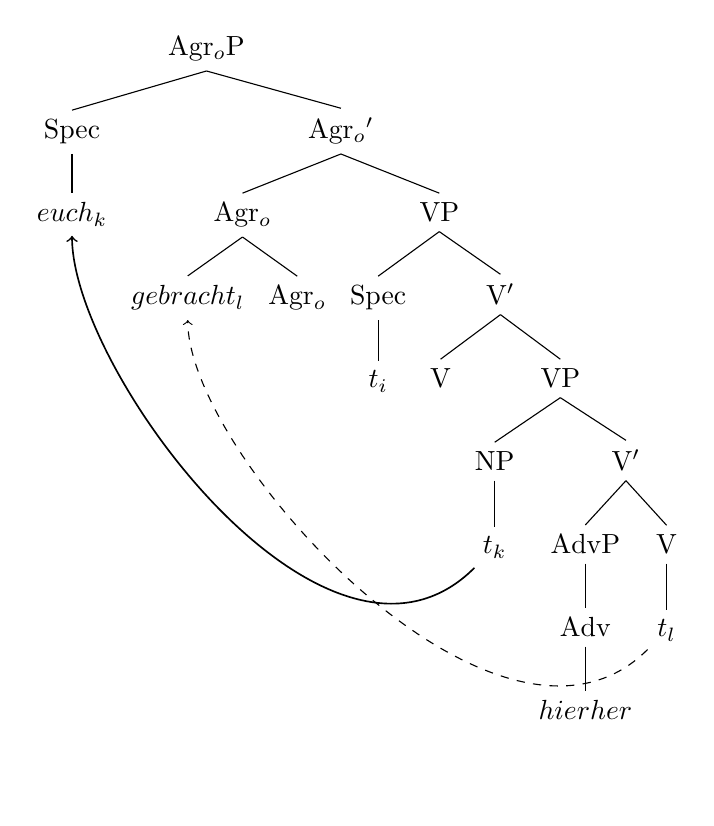
\begin{tikzpicture}
\Tree [.Agr$_o$P
		[.Spec \node(o){$euch_k$}; ] [.Agr$_o$$'$
		[.Agr$_o$ \node(v){$gebracht_l$}; Agr$_o$ ] [.VP
		[.Spec {$t_i$} ] [.V$'$
		V [.VP
		[.NP \node(tk){$t_k$}; ] [.V$'$
		[.AdvP [.Adv {$hierher$} ] ] [.V \node(tl){$t_l$}; ] ] ] ] ] ] ]
\draw[dashed, ->] (tl)..controls +(south west:3) and +(south:2)..(v);
\draw[semithick, ->] (tk)..controls +(south west:3) and +(south:2)..(o);
\end{tikzpicture}\\
}

{\bf Figure 5e. ``Wer hat euch hierher gebracht?'' (Verb tense checking)}\\
\bigskip
{\centering
\begin{tikzpicture}
\Tree [.TP 
		[.T \node(v){$gebracht_l$}; [.T {$t_i$} ] ] [.Agr$_o$P
		[.Spec {$euch_k$} ] [.Agr$_o$$'$
		[.Agr$_o$ \node(tl){$t_l$}; Agr$_o$ ] [.VP
		[.Spec {$t_i$} ] [.V$'$
		V [.VP
		[.NP {$t_k$} ] [.V$'$
		[.AdvP [.Adv {$hierher$} ] ] [.V {$t_l$} ] ] ] ] ] ] ] ]
\draw[semithick, ->] (tl)..controls +(south west:2) and +(south:2)..(v);
\end{tikzpicture}\\
}
\bigskip
\subsection{A Gruesome but Interesting End}
I end by taking a final sentence from the conclusion of the Grimm Brothers' ``H\textipa{\"a}nsel und Gretel", a sentence which is both characteristically gruesome, as German fairy tales are known to do, and interesting for our syntactic purposes. The sentence shown in Figure 6 is ``Die gottlose Hexe mu\ss te elendiglich verbrennen.": 'The godless witch had to burn to death miserably', where the DP {\it die gottlose Hexe} is 'the godless witch', {\it elendiglich} is the adverb 'miserably', and {\it musste verbrennen} is the past tense of the modal construction 'must burn to death', where {\it ver} is a prefix that more or less works as an intensifier or completive. In this case, like the previous example the AdvP is inside of the VP, only the motivation is not so clear as before. We could have gotten the same order had we located the adverb outside of the VP. There is a problem with such a construction, however, and the problem comes when we introduce an anaphor like {\it sich}, which would give the meaning more-or-less: 'she herself had to burn'. In this case the order is {\it ...musste sich elendiglich verbrennen}, suggesting the Adverb must in fact be lower down. Therefore we might rather consider Adverb Phrases to default to VP-internal location, with constructions like we found with the Wh-word {\it wie} adopting an alternative VP-external configuration. \\
\bigskip
{\bf Figure 6a. ``Die gottlose Hexe mu\ss te elendiglich verbrennen.''}\\
\bigskip
{\centering
\begin{tikzpicture}
\Tree [.Agr$_s$P
		Spec [.Agr$_s$$'$ 
		Agr$_s$ [.TP 
		[.T {$mu\ss te$} ] [.Agr$_o$P 
		Agr$_o$ [.VP
		[.Spec [.DP \edge[roof];{\it die gottlose Hexe} ] ] [.V$'$
		[.AdvP [.Adv {$elendiglich$} ] ] [.V {$verbrennen$} ] ] ] ] ] ] ] ]
\end{tikzpicture}\\
}
\bigskip
Additionally, since the subject is a complex DP in this case, it is worth noting the verb's checking of nominative case will apply to the DP as a whole, so that not only will the individual elements of the DP agree with the $\phi$-features of the Noun, but they will also each show matching inflection for whatever case is assigned: in this case Nominative. How such case checking is done is another question, because we already said that DP-internal agreement is post-Spellout due to problems in the relative ordering. So if this is the case, what happens when there is overt case checking between Subject and Verb, but covert agreement within the Subject DP? One possibility which I will adopt here is that when the verb checks case it is rather the checking a kind of case feature present in the DP-internal Agr Phrases, and only later when the internal configurations for agreement checking in the DP commence are each of the constituents of the DP checked for case marking as well.   
\newpage
{\bf Figure 6b. ``Die gottlose Hexe mu\ss te elendiglich verbrennen.'' (S-V Agr)}\\
\bigskip
{\centering
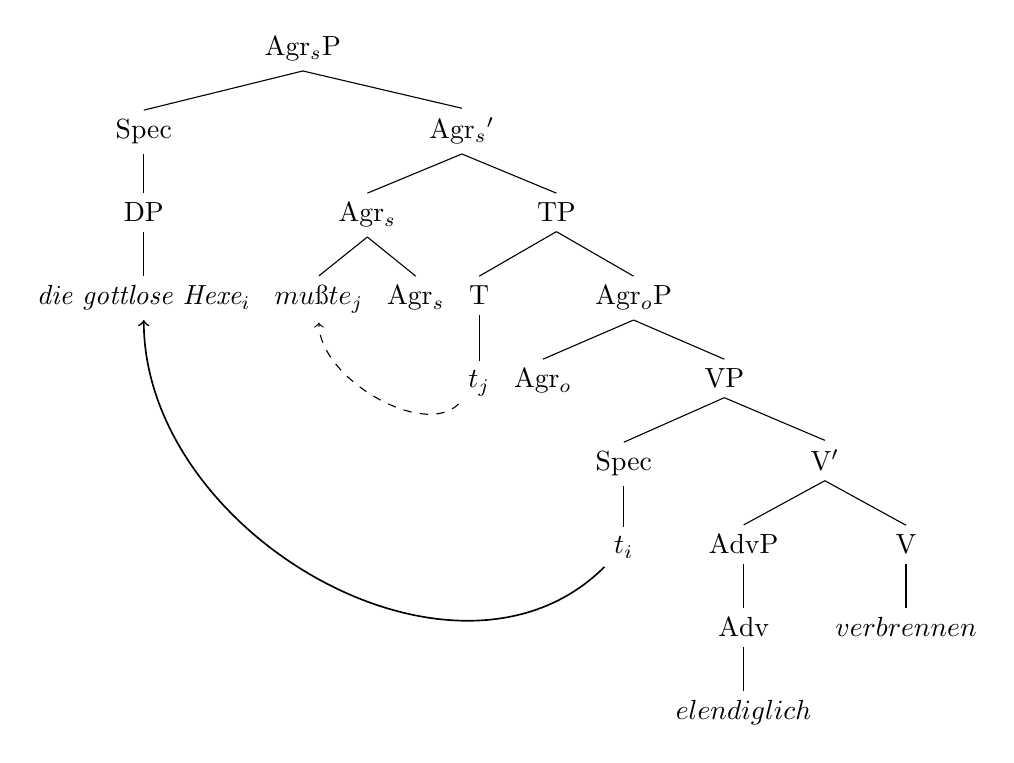
\begin{tikzpicture}
\Tree [.Agr$_s$P
		[.Spec [.DP \node(s){\it die gottlose Hexe$_i$}; ] ] [.Agr$_s$$'$ 
		[.Agr$_s$ \node(v){$mu\ss te_j$}; Agr$_s$ ] [.TP 
		[.T \node(tj){$t_j$}; ] [.Agr$_o$P 
		Agr$_o$ [.VP
		[.Spec \node(ti){$t_i$}; ] [.V$'$
		[.AdvP [.Adv {$elendiglich$} ] ] [.V {$verbrennen$} ] ] ] ] ] ] ]
\draw[dashed, ->] (tj)..controls +(south west:1) and +(south:1)..(v);
\draw[semithick, ->] (ti)..controls +(south west:3) and +(south:3)..(s);
\end{tikzpicture}\\
}
\bigskip
\section{Conclusion}
While the basics of German agreement boil down to two relations -- DP-internal and Verb-Subject (excluding case checking as not 'agreement' as such but rather a separate checking procedure within the AgrP configuration) -- we have seen that the interaction between these two relations is more complex and perhaps not well accounted for at this point. Additionally, I have argued for an SOV structure VP-internally, which nevertheless leads to split word-order configurations in German (i.e. SVO in simple clauses but otherwise V2 auxiliary with a stranded main verb / participle at the end of the clause). Thus the motivation for OV rather than VO comes from this requirement that when TP projects an auxiliary of some sort in its head position overt movement of the lower verb is no longer motivated, meaning the VP-internal order in such cases must be the one which surfaces after Spellout. Other issues such as the varied positioning of Adverbial Phrases and the explanation of V2 patterns have been given partial solutions, but perhaps there are finer details which are not fully resolved. Inspection of more complex clauses is certainly required to test the present model more fully.  

\newpage
\bibliographystyle{plain}
\begin{thebibliography}{9}
\bibitem{chomsky}
	Chomsky, N.
	(1995).
	{\it The Minimalist Program}
	Cambridge University Press,
	Cambridge.
\bibitem{grimm}
  	Godwin-Jones, R.
	(1999).
  	{\it Fairy tales by the Grimm brothers}.
  	Virginia Commonwealth University.
  	http://www.fln.vcu.edu/grimm/.
\end{thebibliography}

\end{flushleft}
\end{document}